\chapter{Scale, Flow, and the Arithmetic of Durable Wealth}

This chapter comes from a School of Hard Knocks conversation with Grant Cardone, curated into companion-note form by LazyingArt LLC with Video2Book. It is not a formal lecture in economics, but it is structured by a real and persistent arithmetic: how much money exists, how little a million dollars can do when spread over time, how scale changes the behavior of a business, and how durable wealth differs from temporary income. The interview moves by rough calculations, state changes, and worked examples. We will keep that movement.

\section{A Tiny Slice of a Huge Money Pool}

The lecture begins before the host introduction, and the beginning matters. Cardone does not open with biography, with ethics, or with advice about self-esteem. He opens with a pipeline: build an audience, make offers, and invite that audience into investment. The first mathematical object is therefore not salary, but scale.

He says that he has raised \$1.1 billion by crowdfunding on the internet, and he places that achievement against what he takes to be the relevant denominator: roughly \$80 trillion of U.S. dollars in circulation. The point is not a monetary theory. The point is a way of measuring ambition.

\begin{equation}
T_{\$}=80\times 10^{12},
\qquad
s(W)=\frac{W}{T_{\$}}.
\end{equation}

Here \(T_{\$}\) denotes the total dollar pool he invokes, and \(s(W)\) is the share of that pool represented by a target wealth \(W\). If we push his rhetoric into explicit arithmetic, we get

\begin{align}
s(10^6) &= \frac{10^6}{80\times 10^{12}} = 1.25\times 10^{-8},\\
s(10^9) &= \frac{10^9}{80\times 10^{12}} = 1.25\times 10^{-5}.
\end{align}

These are not equations from a board. They are clean reconstructions of the lecture's opening move. A million dollars and even a billion dollars are re-described not as the whole of the universe, but as tiny claims on an enormous stock. Once one thinks this way, the phrase ``I need a tiny piece'' stops being rhetoric and becomes a scaling instruction.

This opening also introduces a second theme that will return later: if the relevant pool is enormous, then the problem is not merely accumulation. It is access. Money must come through channels, and those channels must be built.

\section{Boredom, Urgency, and the Destruction Loop}

Only after the cold open does the interview reset into its first explicit question: free time, distraction, addiction, and self-improvement. Cardone's answer is not especially delicate, but it is structurally precise. He gives us a causal chain. Boredom is not merely unpleasant; it is the condition under which compromise becomes likely.

\begin{equation}
\text{boredom} \to \text{compromise} \to \text{trouble},
\qquad
\text{urgency} \to \text{schedule} \to \text{production}.
\end{equation}

That crude diagram captures more of the lecture than one might think at first hearing. The interview is about money, but the money argument presupposes repeated competent action over long stretches of time. One does not ``make a billion'' by a single stroke. One remains available to production, or one drifts into destruction. Hence the early emphasis on sleep, waking early, workouts, breakfast meetings, and surrounding oneself with people who are already moving.

The point of this section is therefore preparatory. Before Cardone asks how many million-dollar wins are needed to keep a billion dollars, he asks whether one has built a life that can even sustain repeated effort. The lecture's moralism is inseparable from its arithmetic.

\section{A Million Dollars Is Still No Money}

The interview now raises the first clean numerical question. The host recalls Cardone's claim that living on a million dollars is not wealth but worry. Here the lecture slows down and does actual counting.

\subsection{Question \& Answer}

\paragraph{Question.}
Why is a million dollars not yet freedom?

\paragraph{Answer.}
Cardone answers by converting a stock of money into a monthly spending flow. He asks the listener's age, asks how long the listener expects to live, and then performs the division that changes the emotional meaning of the number.

If we follow the numbers given in the interview, we have current age \(21\), terminal age \(80\), and therefore

\begin{align}
N_m &= (80-21)\times 12 = 708,\\
\frac{1{,}000{,}000}{N_m} &\approx \frac{1{,}000{,}000}{708} \approx 1{,}412\ \text{USD/month}.
\end{align}

This is the worked example around which the whole section turns. The listener has not yet made a mistake, has not yet paid for an emergency, and has not yet suffered inflation. Nevertheless the monthly spending level is already narrow. The lecture's conclusion is immediate: a million dollars is too thin a cushion to count as freedom.

The interview then pushes the same demystification upward. Cardone asks how many times one must make and retain a million dollars in order to keep a billion. A clean way to formalize his remark is to let \(r\) be the retained fraction of each gross \$1 million after taxes, payroll, and all other leakage. Then the number of required gross million-dollar wins is

\begin{equation}
N_{\text{gross million wins}}=\frac{10^9}{r\cdot 10^6}=\frac{1000}{r}.
\end{equation}

If \(r\) is modest, the number of repetitions is indeed in the thousands. This is not his exact spoken equation, but it is the faithful mathematical spine of what he means by ``thousands and thousands of times, and not blow it.''

The lecture uses this arithmetic to attack a reference-point error. People think a million is large because someone once taught them that it was large. The calculation is meant to break that inheritance.

\section{From Poor to Rich to Wealthy}

Once the million-dollar prestige has been punctured, the lecture broadens into a taxonomy. The key distinction is not between poor and rich alone, but between rich and wealthy.

\begin{definition}
In the working vocabulary of this interview, \emph{rich} means high present income tied to a person or a job, while \emph{wealthy} means a structure of assets, enterprise, or brand that can continue when the original operator disappears.
\end{definition}

The lecture describes a path through states:

\begin{equation}
\text{poor}\to\text{middle class}\to\text{rich}\to\text{wealthy}.
\end{equation}

The middle class appears here not as a stable achievement but as a temptation: one has air conditioning, a car, some entertainment, perhaps a bottle on the weekend, and enough distance from earlier poverty to believe the problem is solved. Rich comes next: a large salary, taxes, house, country-club markers, the appearance of success. But the lecture insists that this still may not be freedom.

The proof is autobiographical. Cardone's father dies, the income stops, and within days the family's situation changes. In the interview this is not a mere story. It is the local demonstration that high inflow is not the same thing as durable structure.

\begin{figure}[h]
\centering
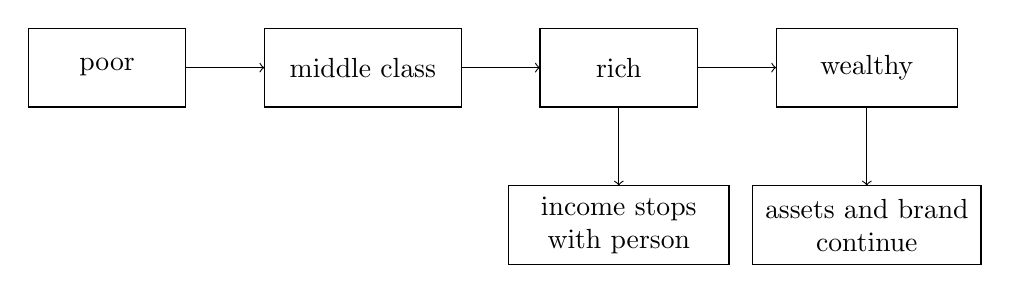
\begin{tikzpicture}[x=1cm,y=1cm]
\draw (0,0) rectangle (2,1);
\node at (1,0.5) {poor};

\draw (3,0) rectangle (5.5,1);
\node at (4.25,0.5) {middle class};

\draw (6.5,0) rectangle (8.5,1);
\node at (7.5,0.5) {rich};

\draw (9.5,0) rectangle (11.8,1);
\node at (10.65,0.5) {wealthy};

\draw[->] (2,0.5) -- (3,0.5);
\draw[->] (5.5,0.5) -- (6.5,0.5);
\draw[->] (8.5,0.5) -- (9.5,0.5);

\draw (6.1,-2) rectangle (8.9,-1);
\node[align=center] at (7.5,-1.5) {income stops\\with person};
\draw[->] (7.5,0) -- (7.5,-1);

\draw (9.2,-2) rectangle (12.1,-1);
\node[align=center] at (10.65,-1.5) {assets and brand\\continue};
\draw[->] (10.65,0) -- (10.65,-1);
\end{tikzpicture}
\end{figure}

This diagram states the lecture's central structural claim. Rich can die with the person. Wealth, if it is real, is designed not to.

\section{The Way to Money Is Through People}

Having classified states of wealth, the interview pivots to mechanism. The mechanism is simple enough to be almost embarrassing: money comes through people.

\begin{definition}
The conduit principle of the lecture is this: money does not arrive in a human life except through another human being.
\end{definition}

The credit-card demonstration makes the point in miniature. One can either steal once, or one can build a relationship and open a repeated channel. The channel is the substance. That principle then scales upward into audience-building, fundraising, sales, and brand.

The same logic organizes the section on \emph{Undercover Billionaire}. Cardone is given \$100 and asked to build a business. His response is not to manage the \$100 carefully. It is to reject the frame altogether. The lecture's reasoning is that if the target is \$10 million, then the right problem is not how to protect the initial \$100, but how to reach people at scale. Hence the slogan: get to zero fast, stop thinking like a manager of tiny sums, and start thinking like someone who raises and deploys capital.

\begin{figure}[h]
\centering
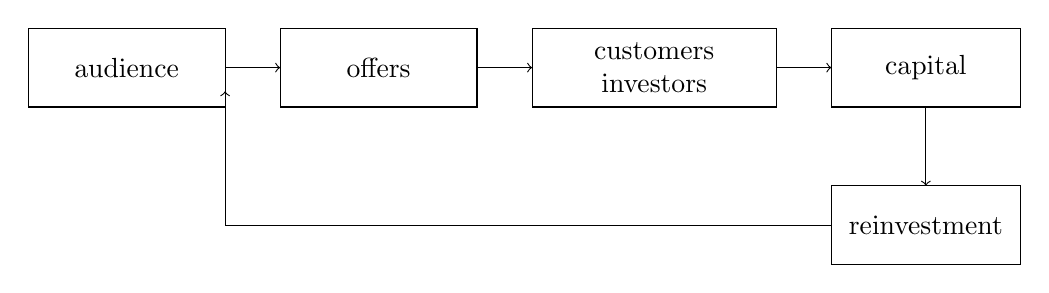
\begin{tikzpicture}[x=1cm,y=1cm]
\draw (0,0) rectangle (2.5,1);
\node[align=center] at (1.25,0.5) {audience};

\draw (3.2,0) rectangle (5.7,1);
\node[align=center] at (4.45,0.5) {offers};

\draw (6.4,0) rectangle (9.5,1);
\node[align=center] at (7.95,0.5) {customers\\investors};

\draw (10.2,0) rectangle (12.6,1);
\node[align=center] at (11.4,0.5) {capital};

\draw (10.2,-2) rectangle (12.6,-1);
\node[align=center] at (11.4,-1.5) {reinvestment};

\draw[->] (2.5,0.5) -- (3.2,0.5);
\draw[->] (5.7,0.5) -- (6.4,0.5);
\draw[->] (9.5,0.5) -- (10.2,0.5);
\draw[->] (11.4,0) -- (11.4,-1);
\draw[->] (10.2,-1.5) -- (2.5,-1.5) -- (2.5,0.2);
\end{tikzpicture}
\end{figure}

The figure is a transcript-based reconstruction of the interview's operating logic. Audience leads to offers, offers lead to customers or investors, and the resulting capital is not meant to be stacked inertly. It is meant to be sent back into the machine.

That is why the lecture joins capital to brand-building. One keeps showing up, keeps making noise, keeps learning in public, and keeps being present enough that people cannot ignore the existence of the channel. The high-school story about the man who never won a fight but always showed up serves exactly this purpose: repetition changes the field even before excellence arrives.

\section{One House Does Not Scale}

The interview now reaches its most concrete business example: real estate. Here again the host's first formulation is corrected by the speaker. The host suggests a jump from one unit to a much larger second deal. Cardone replies that the first two deals were single-family houses and that the large leap came on the third deal, a 48-unit property. That correction matters, because it preserves the lecture's actual rhythm: experiment, discovery of the bottleneck, study, then scaled action.

\subsection{Question \& Answer}

\paragraph{Question.}
Why does a single house fail as a scalable wealth machine?

\paragraph{Answer.}
Because the cash flow is too local and too fragile. One tenant leaves, and the income may collapse to zero.

Cardone gives a miniature example. A tenant moves in, pays, then moves out, and there is no money. That observation leads him to the sentence that organizes the whole section: do not buy one unit.

The first single-family deal nevertheless teaches something. It produces about \$200 per month of cash flow and thereby reveals that sales is not the only way to generate income. But the lecture insists that this is still insufficient because the system does not scale.

When the 48-unit deal arrives, the arithmetic changes orders of magnitude. The secure quantities stated in the interview are these: roughly \$350{,}000 raised, a \$1.9 million note signed, and roughly \$3.7 million net on the deal.

\begin{align}
E &= 350{,}000,\\
D &= 1.9\times 10^6,\\
P &\approx 3.7\times 10^6.
\end{align}

From these numbers we may compute a derived metric, while remaining careful not to infer more structure than the transcript supports:

\begin{equation}
\frac{P}{E}\approx \frac{3.7\times 10^6}{350{,}000}\approx 10.6.
\end{equation}

This is not a number Cardone states directly. It is simply the explicit ratio hiding inside the figures he gives. It explains why the deal becomes the decisive break in the story.

The lecture immediately extends that arithmetic into a naive but revealing update rule:

\begin{equation}
10\cdot P \approx 10\cdot 3.7\times 10^6 = 3.7\times 10^7.
\end{equation}

This is how the imagination shifts. One does not yet think of 12,000 units, the internet, or a fleet of businesses. One thinks first of doing the same scalable thing several times.

\begin{remark}
One line in this portion of the transcript about the 48-unit asset ``earning \$48,000 a month'' and ``making \$1,000'' is garbled. It is safer to retain only the quantities that are clearly spoken. Likewise, the financing point should be stated conceptually: in the lecture, the loan is attached to the apartment LLC and the asset structure, not primarily to a personal retail credit score.
\end{remark}

\begin{figure}[h]
\centering
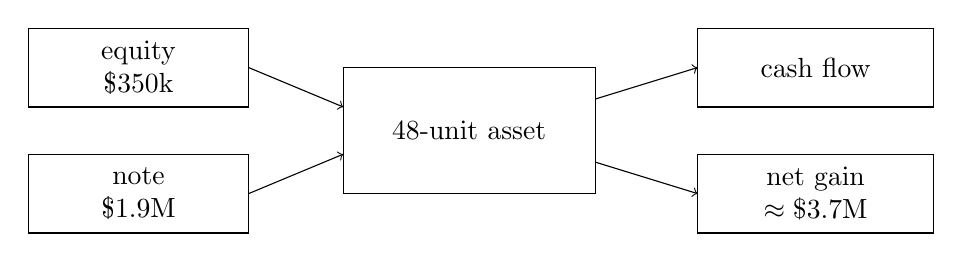
\begin{tikzpicture}[x=1cm,y=1cm]
\draw (0,0.8) rectangle (2.8,1.8);
\node[align=center] at (1.4,1.3) {equity\\\$350k};

\draw (0,-0.8) rectangle (2.8,0.2);
\node[align=center] at (1.4,-0.3) {note\\\$1.9M};

\draw (4,-0.3) rectangle (7.2,1.3);
\node[align=center] at (5.6,0.5) {48-unit asset};

\draw (8.5,0.8) rectangle (11.5,1.8);
\node[align=center] at (10,1.3) {cash flow};

\draw (8.5,-0.8) rectangle (11.5,0.2);
\node[align=center] at (10,-0.3) {net gain\\\(\approx \$3.7\)M};

\draw[->] (2.8,1.3) -- (4,0.8);
\draw[->] (2.8,-0.3) -- (4,0.2);
\draw[->] (7.2,0.9) -- (8.5,1.3);
\draw[->] (7.2,0.1) -- (8.5,-0.3);
\end{tikzpicture}
\end{figure}

\section{Scale, Conversion, and the Endgame}

Before the ad break, the lecture widens again. Commitment matters more than excuses. Assets matter more than credit scores. Demand should be read where it actually appears. That is why the interview briefly tours lottery spending, visible abs, billionaires, yachts, and fishing boats. At first these examples seem disconnected. They are not. They are all attempts to say the same thing: go where the flow is large enough to matter.

Two quantities are especially clean. First, lottery spending:

\begin{equation}
L = 105\times 10^9\ \text{USD/year}.
\end{equation}

Cardone uses this not as a moral endorsement of the lottery, but as evidence that enormous sums accumulate around what people visibly want. Second, the ratio between American millionaires and Americans with visible abs:

\begin{equation}
\frac{22\times 10^6}{3\times 10^6}=\frac{22}{3}\approx 7.33.
\end{equation}

Again the purpose is not physiological truth but probability reframing. The same mind that says ``follow the money'' on the sea, by following where the largest yachts cluster, says here: follow the large counts.

After the interruption the lecture restarts with a harder sentence: if one does not scale, one does not really have a business. Small organizations are controlled by their customers, their employees, and finally by the owner's own exhaustion. Large organizations can absorb local loss. This point then flows directly into talent, trust, and sales.

Cardone's sales arithmetic comes in two layers. The first is structural: 80\% of what he does is free, 20\% pays, and the free layer is not waste but funnel. The second is numerical. The transcript gives counts for interested investors, actual investors, buyers, and repeat buyers. The spoken percentages are inconsistent, so the faithful note must preserve the counts and correct the arithmetic.

\begin{align}
c_{\text{invest}} &= \frac{13{,}000}{450{,}000} \approx 2.89\%,\\
c_{\text{buy}} &= \frac{154{,}000}{16{,}000{,}000} \approx 0.96\%,\\
c_{\text{repeat}} &= \frac{45{,}000}{154{,}000} \approx 29.2\%.
\end{align}

What matters here is not merely conversion. It is the lecture's redefinition of closing. To close is not, in his language, to trap the buyer. It is to serve the buyer for the first time. That is why the repeat-purchase count matters. A close is not the end of a process but the moment the relationship becomes active.

The final movement of the interview brings the arithmetic back down into a life. Cardone speaks about recovery, the years of showing up first and leaving last, the refusal to go to a birthday party at 2:30 in the morning, and the deliberate manufacture of dissatisfaction in order to remain in motion. The point is that the large flows above do not excuse routine. They depend on routine.

The closing investment rule is therefore simple:

\begin{equation}
\text{earn} \to \text{reinvest in self, business, brand} \to \text{acquire outside real assets}.
\end{equation}

This sequence also lets us interpret the lecture's final insistence that money is important. Institutions, hospitals, stores, schools, churches, and families do not accept ``happy moments'' as payment. They take dollars. The arithmetic of production is therefore not opposed to responsibility. In the interview it is responsibility.

At the end he makes a concrete market call on Austin real estate, even forecasting sharp discounts relative to prior purchase prices. That forecast should be heard as a dated market judgment, not as a theorem. The durable part of the section lies elsewhere: money should not simply be stored, and the system should eventually point beyond one's own operating business toward real assets that stand outside it.

\section{Summary}

The lecture begins with an enormous denominator and ends with a daily schedule. Between those points it constructs a compact theory of wealth. A million dollars becomes monthly spending and therefore loses its mystique. Rich and wealthy separate once we ask whether income survives the person. Money is said to travel through people, not around them. Small deals teach, but scalable structures transform. Free attention becomes paid conversion. And the whole machine depends on a life organized against boredom and in favor of repeated production.

The mathematics here is elementary by design. That is why it matters. The interview's wager is that if we keep the ratios, the flows, and the state changes in view, the world of wealth begins to look less like luck and more like structure.